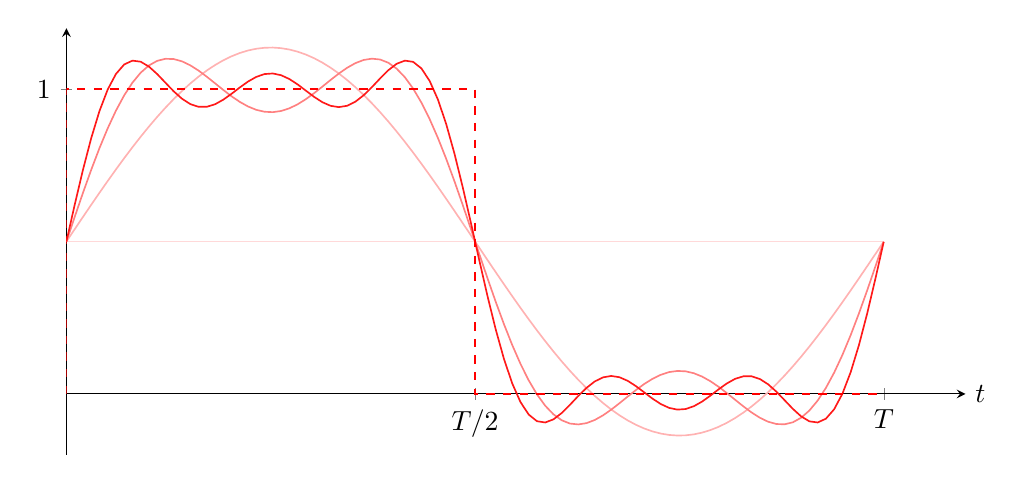
\begin{tikzpicture}
\begin{axis}[
    width=13cm, 
    height=7cm,
    axis x line=center, 
    axis y line=middle, 
    xlabel={$t$},
     x label style={at={(current axis.right of origin)}, right},
    samples=100,
    ymin=-0.2, ymax=1.2,
    xmin= 0, xmax=1.1,
    domain=0:1,
    xtick={   0.5,  1  },
    xticklabels={ $T/2$ , $T$ }, 
    ytick={0, 1},
    yticklabels={$0$, $1$}
]
\addplot [mark=none, semithick, red!15!white] {0.5};   %sin(deg(x))
\addplot [mark=none, semithick, red!30!white] {0.5+(2/pi)*sin(deg(2*pi*x))};   
\addplot [mark=none, semithick, red!50!white] {0.5+(2/pi)*sin(deg(2*pi*x))+(2/(3*pi))*sin(deg(6*pi*x))};   
\addplot [mark=none, semithick, red!90!white] {0.5+(2/pi)*sin(deg(2*pi*x))+(2/(3*pi))*sin(deg(6*pi*x))++(2/(5*pi))*sin(deg(10*pi*x))};   %
\draw[red, dashed, semithick] (axis cs: 0, 0) -- (axis cs: 0, 1) -- (axis cs: 0.5, 1) -- (axis cs: 0.5, 0) -- (axis cs: 1, 0);
\end{axis}
\end{tikzpicture}
